%% Source: https://github.com/tias/constraint-solving-course
%% Licensed under CC BY-NC-SA 4.0: https://creativecommons.org/licenses/by-nc-sa/4.0/
%% You may share and adapt this for non-commercial use,
%% with attribution and under the same license.

\documentclass{cons-beamer}

\begin{document}


\begin{frame}{L03: Solving, debugging and explanation techniques}
  \begin{center}
    ~ \\
    \includegraphics[height=42mm]{images/texpl_img/interaction_figure4.png} \\
    Prof. Tias Guns and Dr. Dimos Tsouros \\[0.5em]
    \includegraphics[width=2cm]{images/kuleuven_CMYK_logo.pdf}
  \end{center}
  
  {\footnotesize 
  Partly based on slides from Pierre Flener, Uppsala University.}
  % https://pierre-flener.github.io/courses/M4CO/lectures.html
\end{frame}


\section{Solving the problem}

\begin{frame}{Model + \textbf{Solve}}

  Declarative problem solving: We model \textbf{what} -- the solver takes care of the \textbf{how} \dots   \vfill

  We saw how to model a combinatorial problem in a CP modeling language... 
  \vfill

  Now, we want to \textit{solve} it! \vfill
  
  Combinatorial problems:
  \begin{itemize}
    \item  Huge \red{search space}
    \item \red{Exponential} growth of possible solutions
    \begin{itemize}
      \item For \( n \) variables with \( d \) possible values each, the \red{search space size is \( d^n \)}
    \end{itemize}
    \item Inference based on the constraints helps to prune infeasible solutions early, \inference{reducing the search space}
  \end{itemize}
\end{frame}

\begin{frame}{Solving combinatorial problems}
  
  Combinatorial problems: Huge \red{search space}
  \vfill

% Huge Search Space without Constraints
\scriptsize	
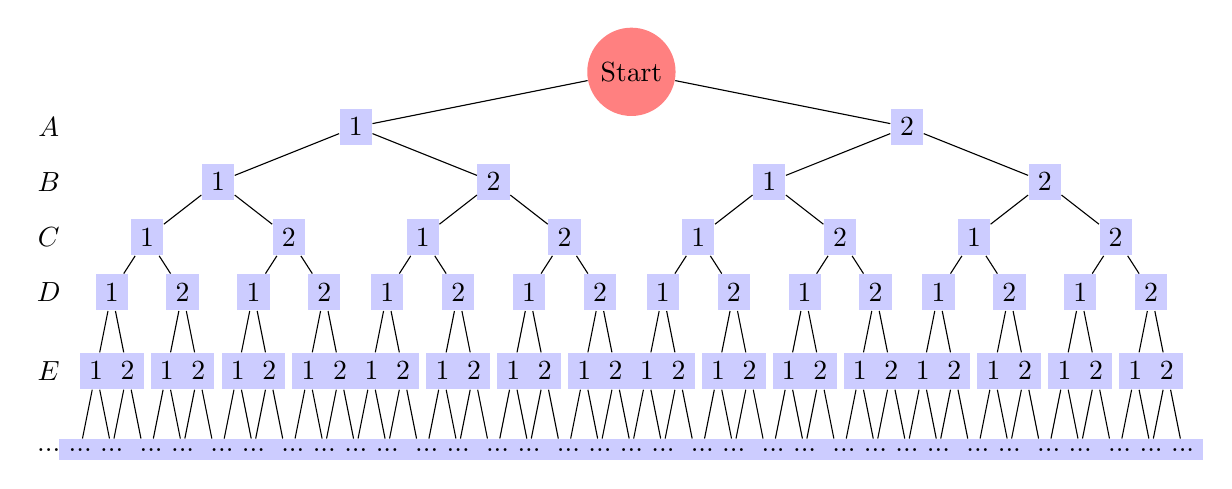
\begin{tikzpicture}[
val/.style={rectangle, fill=blue!20},
root/.style={circle, fill=red!50},
var/.style={rectangle},
level 1/.style={level distance=0.7cm, sibling distance=7cm},
level 2/.style={level distance=0.7cm, sibling distance=3.5cm},
level 3/.style={level distance=0.7cm, sibling distance=1.8cm},
level 4/.style={level distance=0.7cm, sibling distance=0.9cm},
level 5/.style={level distance=1cm, sibling distance=0.4cm},
]

% Variables listed on the side
\coordinate (V) at (-7.4,0);
\node[var] at (V) { };
\coordinate (A) at (-7.4,-0.7);
\node[var] at (A) {$A$};
\coordinate (B) at (-7.4,-1.4);
\node[var] at (B) {$B$};
\coordinate (C) at (-7.4,-2.1);
\node[var] at (C) {$C$};
\coordinate (D) at (-7.4,-2.8);
\node[var] at (D) {$D$};
\coordinate (E) at (-7.4,-3.8);
\node[var] at (E) {$E$};
\coordinate (E) at (-7.4,-4.8);
\node[var] at (E) {...};

% Root node and expanded search space with values only
\node[root] {Start} 
  child{node[val]{1} % A=1
    child{node[val]{1} % B=1
      child{node[val]{1} % C=1
        child{node[val]{1} % D=1
          child{node[val]{1}
           child{node[val]{...}}
           child{node[val]{...}}           
           } % E=1
          child{node[val]{2}
           child{node[val]{...}}
           child{node[val]{...}}  
           } % E=2
        }
        child{node[val]{2} % D=2
          child{node[val]{1}
         child{node[val]{...}}
           child{node[val]{...}}
           } % E=1
          child{node[val]{2}
           child{node[val]{...}}
           child{node[val]{...}}  
           } % E=2
        }
      }
      child{node[val]{2} % C=2
        child{node[val]{1} % D=1
          child{node[val]{1}
           child{node[val]{...}}
           child{node[val]{...}}           
           } % E=1
          child{node[val]{2}
           child{node[val]{...}}
           child{node[val]{...}}  
           } % E=2
        }
        child{node[val]{2} % D=2
          child{node[val]{1}
           child{node[val]{...}}
           child{node[val]{...}}           
           } % E=1
          child{node[val]{2}
           child{node[val]{...}}
           child{node[val]{...}}  
           } % E=2
        }
      }
    }
    child{node[val]{2} % B=2
      child{node[val]{1} % C=1
        child{node[val]{1} % D=1
          child{node[val]{1}
           child{node[val]{...}}
           child{node[val]{...}}           
           } % E=1
          child{node[val]{2}
           child{node[val]{...}}
           child{node[val]{...}}  
           } % E=2
        }
        child{node[val]{2} % D=2
          child{node[val]{1}
           child{node[val]{...}}
           child{node[val]{...}}           
           } % E=1
          child{node[val]{2}
           child{node[val]{...}}
           child{node[val]{...}}  
           } % E=2
        }
      }
      child{node[val]{2} % C=2
        child{node[val]{1} % D=1
          child{node[val]{1}
           child{node[val]{...}}
           child{node[val]{...}}           
           } % E=1
          child{node[val]{2}
           child{node[val]{...}}
           child{node[val]{...}}  
           } % E=2
        }
        child{node[val]{2} % D=2
          child{node[val]{1}
           child{node[val]{...}}
           child{node[val]{...}}           
           } % E=1
          child{node[val]{2}
           child{node[val]{...}}
           child{node[val]{...}}  
           } % E=2
        }
      }
    }
  }
  child{node[val]{2} % A=2
    child{node[val]{1} % B=1
      child{node[val]{1} % C=1
        child{node[val]{1} % D=1
          child{node[val]{1}
           child{node[val]{...}}
           child{node[val]{...}}           
           } % E=1
          child{node[val]{2}
           child{node[val]{...}}
           child{node[val]{...}}  
           } % E=2
        }
        child{node[val]{2} % D=2
          child{node[val]{1}
           child{node[val]{...}}
           child{node[val]{...}}           
           } % E=1
          child{node[val]{2}
           child{node[val]{...}}
           child{node[val]{...}}  
           } % E=2
        }
      }
      child{node[val]{2} % C=2
        child{node[val]{1} % D=1
          child{node[val]{1}
           child{node[val]{...}}
           child{node[val]{...}}           
           } % E=1
          child{node[val]{2}
           child{node[val]{...}}
           child{node[val]{...}}  
           } % E=2
        }
        child{node[val]{2} % D=2
          child{node[val]{1}
           child{node[val]{...}}
           child{node[val]{...}}           
           } % E=1
          child{node[val]{2}
           child{node[val]{...}}
           child{node[val]{...}}  
           } % E=2
        }
      }
    }
    child{node[val]{2} % B=2
      child{node[val]{1} % C=1
        child{node[val]{1} % D=1
          child{node[val]{1}
           child{node[val]{...}}
           child{node[val]{...}}           
           } % E=1
          child{node[val]{2}
           child{node[val]{...}}
           child{node[val]{...}}  
           } % E=2
        }
        child{node[val]{2} % D=2
          child{node[val]{1}
           child{node[val]{...}}
           child{node[val]{...}}           
           } % E=1
          child{node[val]{2}
           child{node[val]{...}}
           child{node[val]{...}}  
           } % E=2
        }
      }
      child{node[val]{2} % C=2
        child{node[val]{1} % D=1
          child{node[val]{1}
           child{node[val]{...}}
           child{node[val]{...}}           
           } % E=1
          child{node[val]{2}
           child{node[val]{...}}
           child{node[val]{...}}  
           } % E=2
        }
        child{node[val]{2} % D=2
          child{node[val]{1}
           child{node[val]{...}}
           child{node[val]{...}}           
           } % E=1
          child{node[val]{2}
           child{node[val]{...}}
           child{node[val]{...}}  
           } % E=2
        }
      }
    }
  };

\end{tikzpicture}

\end{frame}


\begin{frame}{Solving combinatorial problems}
  
        \begin{transparent}{0.3}
            Combinatorial problems: Huge \red{search space},
        \end{transparent} \textbf{need \inference{intelligent} \search{search}!}
  \vfill
  
% Reduced Search Space with Constraints
\scriptsize	
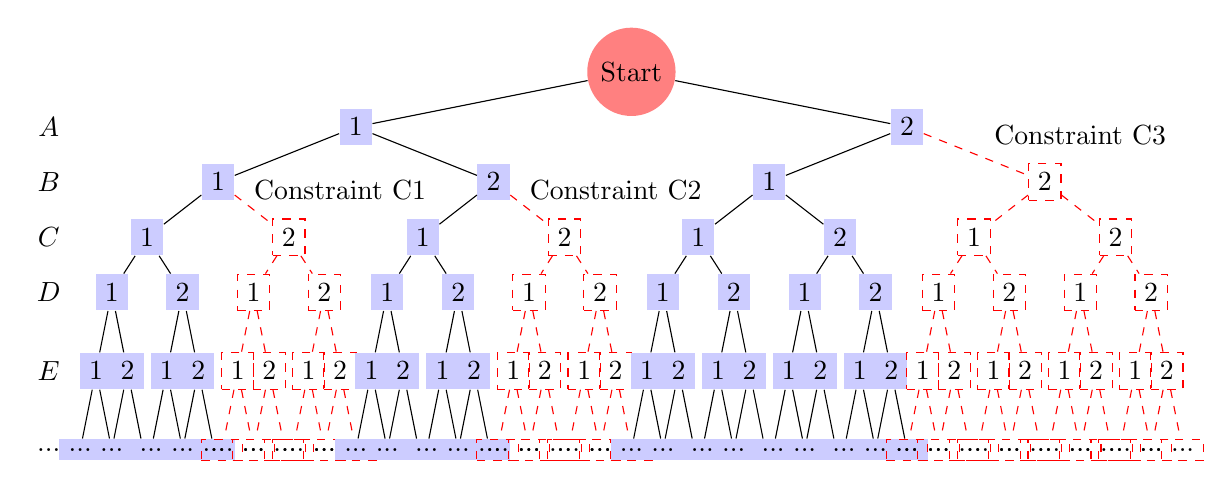
\begin{tikzpicture}[
val/.style={rectangle, fill=blue!20},
root/.style={circle, fill=red!50},
var/.style={rectangle},
pruned/.style={rectangle, draw=red, dashed},
level 1/.style={level distance=0.7cm, sibling distance=7cm},
level 2/.style={level distance=0.7cm, sibling distance=3.5cm},
level 3/.style={level distance=0.7cm, sibling distance=1.8cm},
level 4/.style={level distance=0.7cm, sibling distance=0.9cm},
level 5/.style={level distance=1cm, sibling distance=0.4cm},
]

% Variables listed on the side
\coordinate (V) at (-7.4,0);
\node[var] at (V) { };
\coordinate (A) at (-7.4,-0.7);
\node[var] at (A) {$A$};
\coordinate (B) at (-7.4,-1.4);
\node[var] at (B) {$B$};
\coordinate (C) at (-7.4,-2.1);
\node[var] at (C) {$C$};
\coordinate (D) at (-7.4,-2.8);
\node[var] at (D) {$D$};
\coordinate (E) at (-7.4,-3.8);
\node[var] at (E) {$E$};
\coordinate (E) at (-7.4,-4.8);
\node[var] at (E) {...};

% Root node and expanded search space with values only
\node[root] {Start} 
  child{node[val]{1} % A=1
    child{node[val]{1} % B=1
      child{node[val]{1} % C=1
        child{node[val]{1} % D=1
          child{node[val]{1}
           child{node[val]{...}}
           child{node[val]{...}}           
           } % E=1
          child{node[val]{2}
           child{node[val]{...}}
           child{node[val]{...}}  
           } % E=2
        }
        child{node[val]{2} % D=2
          child{node[val]{1}
         child{node[val]{...}}
           child{node[val]{...}}
           } % E=1
          child{node[val]{2}
           child{node[val]{...}}
           child{node[val]{...}}  
           } % E=2
        }
      }
      child[pruned]{node[pruned]{2} % C=2
        child[pruned]{node[pruned]{1} % D=1
          child[pruned]{node[pruned]{1}
           child[pruned]{node[pruned]{...}}
           child[pruned]{node[pruned]{...}}           
           } % E=1
          child[pruned]{node[pruned]{2}
           child[pruned]{node[pruned]{...}}
           child[pruned]{node[pruned]{...}}  
           } % E=2
        }
        child[pruned]{node[pruned]{2} % D=2
          child[pruned]{node[pruned]{1}
           child[pruned]{node[pruned]{...}}
           child[pruned]{node[pruned]{...}}           
           } % E=1
          child[pruned]{node[pruned]{2}
           child[pruned]{node[pruned]{...}}
           child[pruned]{node[pruned]{...}}  
           } % E=2
        }
      }
    }
    child{node[val]{2} % B=2
      child{node[val]{1} % C=1
        child{node[val]{1} % D=1
          child{node[val]{1}
           child{node[val]{...}}
           child{node[val]{...}}           
           } % E=1
          child{node[val]{2}
           child{node[val]{...}}
           child{node[val]{...}}  
           } % E=2
        }
        child{node[val]{2} % D=2
          child{node[val]{1}
           child{node[val]{...}}
           child{node[val]{...}}           
           } % E=1
          child{node[val]{2}
           child{node[val]{...}}
           child{node[val]{...}}  
           } % E=2
        }
      }
      child[pruned]{node[pruned]{2} % C=2
        child[pruned]{node[pruned]{1} % D=1
          child[pruned]{node[pruned]{1}
           child[pruned]{node[pruned]{...}}
           child[pruned]{node[pruned]{...}}           
           } % E=1
          child[pruned]{node[pruned]{2}
           child[pruned]{node[pruned]{...}}
           child[pruned]{node[pruned]{...}}  
           } % E=2
        }
        child[pruned]{node[pruned]{2} % D=2
          child[pruned]{node[pruned]{1}
           child[pruned]{node[pruned]{...}}
           child[pruned]{node[pruned]{...}}           
           } % E=1
          child[pruned]{node[pruned]{2}
           child[pruned]{node[pruned]{...}}
           child[pruned]{node[pruned]{...}}  
           } % E=2
        }
      }
    }
  }
  child{node[val]{2} % A=2
    child{node[val]{1} % B=1
      child{node[val]{1} % C=1
        child{node[val]{1} % D=1
          child{node[val]{1}
           child{node[val]{...}}
           child{node[val]{...}}           
           } % E=1
          child{node[val]{2}
           child{node[val]{...}}
           child{node[val]{...}}  
           } % E=2
        }
        child{node[val]{2} % D=2
          child{node[val]{1}
           child{node[val]{...}}
           child{node[val]{...}}           
           } % E=1
          child{node[val]{2}
           child{node[val]{...}}
           child{node[val]{...}}  
           } % E=2
        }
      }
      child{node[val]{2} % C=2
        child{node[val]{1} % D=1
          child{node[val]{1}
           child{node[val]{...}}
           child{node[val]{...}}           
           } % E=1
          child{node[val]{2}
           child{node[val]{...}}
           child{node[val]{...}}  
           } % E=2
        }
        child{node[val]{2} % D=2
          child{node[val]{1}
           child{node[val]{...}}
           child{node[val]{...}}           
           } % E=1
          child{node[val]{2}
           child{node[val]{...}}
           child{node[val]{...}}  
           } % E=2
        }
      }
    }
    child[pruned]{node[pruned]{2} % B=2
      child[pruned]{node[pruned]{1} % C=1
        child[pruned]{node[pruned]{1} % D=1
          child[pruned]{node[pruned]{1}
           child[pruned]{node[pruned]{...}}
           child[pruned]{node[pruned]{...}}           
           } % E=1
          child[pruned]{node[pruned]{2}
           child[pruned]{node[pruned]{...}}
           child[pruned]{node[pruned]{...}}  
           } % E=2
        }
        child[pruned]{node[pruned]{2} % D=2
          child[pruned]{node[pruned]{1}
           child[pruned]{node[pruned]{...}}
           child[pruned]{node[pruned]{...}}           
           } % E=1
          child[pruned]{node[pruned]{2}
           child[pruned]{node[pruned]{...}}
           child[pruned]{node[pruned]{...}}  
           } % E=2
        }
      }
      child[pruned]{node[pruned]{2} % C=2
        child[pruned]{node[pruned]{1} % D=1
          child[pruned]{node[pruned]{1}
           child[pruned]{node[pruned]{...}}
           child[pruned]{node[pruned]{...}}           
           } % E=1
          child[pruned]{node[pruned]{2}
           child[pruned]{node[pruned]{...}}
           child[pruned]{node[pruned]{...}}  
           } % E=2
        }
        child[pruned]{node[pruned]{2} % D=2
          child[pruned]{node[pruned]{1}
           child[pruned]{node[pruned]{...}}
           child[pruned]{node[pruned]{...}}           
           } % E=1
          child[pruned]{node[pruned]{2}
           child[pruned]{node[pruned]{...}}
           child[pruned]{node[pruned]{...}}  
           } % E=2
        }
      }
    }
  };

% Labels for pruned branches
\node at (-3.7, -1.5) {\inference{Constraint C1}};
\node at (-0.2, -1.5) {\inference{Constraint C2}};
\node at (5.7, -0.8) {\inference{Constraint C3}};

\end{tikzpicture}

\end{frame}

\begin{frame}{Solving combinatorial problems}
  Different solvers/solving technologies can be used for that. They differ in:
  \begin{itemize}
    \item The constraints they support (including global constraints/functions)
    \item How they perform search and propagation (CP vs MIP vs PB vs SAT)
    \item How they guide the search (heuristics, hyper-parameters)
    \item \dots
  \end{itemize}
\end{frame}

\begin{frame}{Encoding to solver-specific input}
  High-level CP modeling languages have to \defined{encode} problems into a solver-specific input format.
  \vfill
  \begin{center}
    \includegraphics[height=60mm]{images/prob2sol.png}
  \end{center}
\end{frame}

\begin{frame}{Model Transformations}
  \begin{columns}

    % Left Column: Diagram
    \begin{column}{0.7\textwidth}
\begin{tikzpicture}[scale=0.65, every node/.style={transform shape}, node distance=0.5cm]

% Model (green box)
\node[draw, fill=green!30, rounded corners, minimum width=2cm, minimum height=1cm] (model) {Model  (high-level modelling language)};

% Decompose-globals (blue box)
\node[draw, fill=blue!20, below=of model, rounded corners, minimum width=3.5cm, minimum height=1cm] (decompose) {decompose globals};
% Flatten (orange box)
\node[draw, fill=blue!20, below=of decompose, rounded corners, minimum width=3.5cm, minimum height=1cm] (flatten) {flatten};
% Linearize (purple box)
\node[draw, fill=blue!20, below=of flatten, rounded corners, minimum width=3.5cm, minimum height=1cm] (linearize) {linearize};
% int2bool (cyan box)
\node[draw, fill=blue!20, below=of linearize, rounded corners, minimum width=3.5cm, minimum height=1cm] (int2bool) {int to bool};
% pb2sat (pink box)
\node[draw, fill=blue!20, below=of int2bool, rounded corners, minimum width=3.5cm, minimum height=1cm] (pb2sat) {pb to sat};

% Low-level mdoels (no fill)
\node[draw, fill=green!30, rounded corners, dotted, minimum height=1cm, minimum width=4cm, right=1cm of decompose, align=left] (smt) {SMT model};
\node[draw, fill=green!30, rounded corners, dotted, minimum height=1cm, minimum width=4cm, right=1cm of flatten, align=left] (cp) {CP model};
\node[draw, fill=green!30, rounded corners, dotted, minimum width=4cm, right=1cm of linearize, fill=green!30, rounded corners, align=left] (ilp) {ILP model};
\node[draw, fill=green!30, rounded corners, dotted, minimum height=1cm, minimum width=4cm, right=1cm of int2bool, align=left] (pb) {PB model};
\node[draw, fill=green!30, rounded corners, dotted, minimum height=1cm, minimum width=4cm, right=1cm of pb2sat, align=left] (sat) {(max)SAT model};

% Solvers (no fill)
\node[draw, minimum height=1cm, minimum width=4cm, right=1cm of smt, align=left] (smt2) {SMT solver};
\node[draw, minimum height=1cm, minimum width=4cm, right=1cm of cp, align=left] (cp2) {CP solver};
\node[draw, minimum height=1cm, minimum width=4cm, right=1cm of ilp, align=left] (ilp2) {ILP solver};
\node[draw, minimum height=1cm, minimum width=4cm, right=1cm of pb, align=left] (pb2) {PB solver};
\node[draw, minimum height=1cm, minimum width=4cm, right=1cm of sat, align=left] (sat2) {(max)SAT solver};

% Arrows
\draw[->] (model) -- (decompose); 
\draw[->] (decompose) -- (flatten);
\draw[->] (flatten) -- (linearize);
\draw[->] (linearize) -- (int2bool);
\draw[->] (int2bool) -- (pb2sat);

% Connections to low-level
\draw[->] (decompose.east) -- ++(0.5,0) |- (smt.west);
\draw[->] (flatten.east) -- ++(0.5,0) |- (cp.west);
\draw[->] (linearize.east) -- ++(0.5,0) |- (ilp.west);
\draw[->] (int2bool.east) -- ++(0.5,0) |- (pb.west);
\draw[->] (pb2sat.east) -- ++(0.5,0) |- (sat.west);

% Connections to solvers
\draw[->] (smt.east) -- ++(0.5,0) |- (smt2.west);
\draw[->] (cp.east) -- ++(0.5,0) |- (cp2.west);
\draw[->] (ilp.east) -- ++(0.5,0) |- (ilp2.west);
\draw[->] (pb.east) -- ++(0.5,0) |- (pb2.west);
\draw[->] (sat.east) -- ++(0.5,0) |- (sat2.west);

\end{tikzpicture}
    \end{column}

    % Right Column: solver names
    %\hspace{1cm}
    \begin{column}{0.37\textwidth}
      Exxample solvers: 

      \begin{itemize}
        \item SMT: Z3
        \item CP: Or-Tools, Choco, GCS, Minizinc (modeling lang)
        \item ILP: Gurobi
        \item PB: Exact
        \item SAT: PySAT
      \end{itemize}
    \end{column}
  \end{columns}
\end{frame}    

\begin{flashcardcpmpy}  % XXX does not have a preceding general slide...
\begin{frame}[fragile]{Solving in CPMpy}   % [fragile] to allow \cpminline
  Declarative modeling, easy solving
    
  \footnotesize{\lstinputlisting[language=cpmpy,firstline=5,lastline=14]{models_cpmpy/t3_sudoku.py}}
  \vfill

  Can also specify the solver to use:
  \vfill

  \scriptsize{\cpminline{model.solve("choco")  # use choco solver - needs pychoco package}}

  \scriptsize{\cpminline{model.solve("gurobi")  # use gurobi solver - needs gurobipy package}}
  \vfill

  \normalsize{See what solvers you have in your machine:}
  \vfill

  \scriptsize{\cpminline{cp.SolverLookup.solvernames()}}
\end{frame}
\end{flashcardcpmpy}

\begin{frame}[fragile]{Solving vs solution enumeration}  % [fragile] to allow \verbatim
  Is one solution sufficient? In many problems no!
  \vfill

  Finding all (or multiple) solutions by 'blocking' each found solution:

  \begin{verbatim}
      while solutions_found < solution_limit:
        solve problem
        Add constraint that forbids the exact same solution
  \end{verbatim}
\end{frame}

\begin{flashcardcpmpy}
\begin{frame}{Solving vs solution enumeration -- CPMpy}
  Is one solution sufficient? In many problems no!
  \vfill

  Finding all (or multiple) solutions by 'blocking' each found solution::
  \vfill

  \footnotesize
  \lstinputlisting[language=cpmpy,numbers=none,firstline=16,lastline=23]{models_cpmpy/t3_sudoku.py}
  \normalsize
  \vfill

  or just use \cpminline{model.solveAll()} $\xleftarrow{}$ It returns the amount of solutions found, accessing the solutions:  \footnotesize\url{https://cpmpy.readthedocs.io/en/latest/multiple_solutions.html}
\end{frame}
\end{flashcardcpmpy}


\section{Debugging}

\begin{frame}{Debugging}
  You solve the problem, but \\
  you get an \textbf{error}, \\
  or no error, but also \textbf{no (correct) solution}... \\
  Annoying, you have a \textbf{bug}.
  \vfill

  \Large	
  How do you \textbf{debug} a model?

  \begin{center}
    \includegraphics[height=20mm]{images/texpl_img/debug.jpg}
  \end{center}
\end{frame}

\begin{frame}{Debugging}
  General advise for debugging when modeling from expert modeller\textbf{ Håkan Kjellerstrand}:
  \vfill

  \begin{itemize}
    \item Test the model \textbf{early and often}. This makes it easier to detect problems in the model. \vfill

    \item When a model is not working, \textbf{activate the constraints one by one} (e.g. comment out the other constraints) to test which constraint is the culprit: 
          \vspace{-1.5em}
          \begin{algorithmic}
            \FOR{each constraint $c$ in \textit{Constraints}}
              \STATE print ``Trying:'', $c$
              \STATE \textit{Solve} $c$
            \ENDFOR
          \end{algorithmic}
          \vfill

    \item \textbf{Check the domains} (see lower). The domains should be as small as possible, but not smaller. If they are too large it can take a lot of time to get a solution. If they are too small, then there will be no solution. \vfill
  \end{itemize}
\end{frame}

\begin{flashcardcpmpy}
\begin{frame}{Debugging -- CPMpy}
  General advise for debugging when modeling from expert modeller\textbf{ Håkan Kjellerstrand}:
  \vfill

  \begin{itemize}
    \item Test the model \textbf{early and often}. This makes it easier to detect problems in the model. \vfill

    \item When a model is not working, \textbf{activate the constraints one by one} (e.g. comment out the other constraints) to test which constraint is the culprit. 
    \lstinputlisting[language=cpmpy,basicstyle=\footnotesize,firstline=15,lastline=17]{models_cpmpy/t3_bugged.py}    \vfill

    \item \textbf{Check the domains} (see lower). The domains should be as small as possible, but not smaller. If they are too large it can take a lot of time to get a solution. If they are too small, then there will be no solution. \vfill
  \end{itemize}
\end{frame}
\end{flashcardcpmpy}

\begin{frame}{Debugging}
  The bug can be situated in one of three layers:
  \begin{enumerate}
    \item your model
    \item the modeling library (CPMpy)
    \item the solver
  \end{enumerate}
  \vfill

  Ordered from most likely to least likely!
\end{frame}

\begin{frame}{Bug in the solver}
  You try with the default solver (or another one) and you get an error, or not the desired solution.
  \vfill

  \large
  Use a different solver and observe:
  \normalsize 
  \vfill
  
  \begin{enumerate}
    \item Outcome changes! It was a (rare) solver bug. Report it to the bug tracker of the modeling library or directly to the solver developers!
          \vfill

    \item Outcome is the same! Not a solver error after all \dots
  \end{enumerate}
\end{frame}

\begin{flashcardcpmpy}  % XXX does not have a preceding general slide...
\begin{frame}{Debugging a modeling error -- CPMpy}
  You get an error when you create an expression?  \\ Quirks in Python/CPMpy (from last lecture):
  \vfill
  
  \begin{enumerate}
    \item \textbf{Logical and/or}:
          Use $\&$ and $|$, and make sure to always put the subexpressions in brackets. 
          \vfill

          \begin{example}
            write \cpminline{(x == 1) & (y == 0)} instead of \cpminline{x == 1 & y == 0}. The latter won't work.
            Python will think you meant \cpminline{x == (1 & y) == 0}.
          \end{example}
          \vfill
      
    \item you can write \cpminline{vars_list[other_var]} but you can’t write \cpminline{non_var_list[a_var]}. That is because the vars list knows CPMpy, and the \cpminline{non_var_list} does not. Wrap it: \cpminline{non_var_list = cp.cpm_array(non_var_list)} first.
          \vfill
  
    \item CPMpy overloads all/any/max/min/sum/abs to create expressions with them. Always use \cpminline{cp.sum(v)} instead of \cpminline{sum(v)}. You can also use directly NumPy's \cpminline{v.sum()} instead, if \cpminline{v} is a matrix or tensor.
  \end{enumerate}
\end{frame}

\begin{frame}{Debugging a modeling error -- CPMpy}
  You get an error when you create an expression \dots  But you do not know why!
  \vfill
  
  Print the constraints you create (or the subexpressions), and check that the output matches what you wish to express!
  \vfill

  \begin{example}
    The following: \lstinputlisting[language=cpmpy,basicstyle=\footnotesize,firstline=3,lastline=5]{models_cpmpy/t3_sum.py}    
    will print \cpminline{[(IV0) + (IV2) (IV1) + (IV3)]}
    and you can see that it is not really a sum, but a list!

    Solution: Use \cpminline{cp.sum(x)} instead!
  \end{example}
    
\end{frame}
\end{flashcardcpmpy}


\section{Explainable Constraint Solving}

\begin{frame}{Explainable Constraint Solving}
  You model the problem and you solve!
  \blue{No Error!}
  \vfill

  But also:
  \begin{itemize}
    \item What if the model is \red{UNSAT}?
    \item What if the solution is \red{unexpected}?
    \item What if the solution is \red{not good enough}?
  \end{itemize}
  \vfill

  There is a modeling error \dots
  Or the problem constraints are too tight \dots
  \vfill

  \textbf{Explainable AI}: Human-Aware AI systems that interact with the users to assist in decision making  
\end{frame}

\begin{frame}{Mode of interaction}
  \centering
  \includegraphics[height=60mm]{images/texpl_img/interaction_figure4.png}
\end{frame}

\begin{frame}{Explainable Constraint Solving}
  In general, "Why $X$?"   (with $X$ (part of) a solution or \red{UNSAT})

  2 patterns of explanations:
  \vfill

  \begin{enumerate}
    \item \textbf{Deductive explanation}:
          How was $X$ derived? (Why I didn't get any solution?)
          \vfill

    \item \textbf{Counterfactual explanation}:
          Why $X$ and not $Z$? (How can I make it satisfiable?) 
          \vfill
  \end{enumerate}
\end{frame}

\begin{frame}{Running Example}
  \begin{example}[Graph Colouring]
    \footnotesize	
    Graph colouring is the problem of assigning colours to the nodes of a graph, such that no two \textbf{adjacent} nodes share the same colour. 

    \begin{itemize}
      \item Variables are the nodes, possible values are the colours: 
            $\text{node}_i \in \{1, 2, \dots, \text{max\_colors}\}, \quad \forall i \in \text{Nodes}$
      \item Constrain edges to have differently colored nodes (i.e., not equal values):
            $\text{node}_{1} \neq \text{node}_{2}, \quad \forall (\text{node}_1, \text{node}_2) \in \text{Edges}$ 
    \end{itemize}
  \end{example}

  \vspace{-0.4cm}
  \footnotesize	
  \begin{columns}
    \begin{column}{0.45\textwidth}
      \begin{center}
        Initial graph:

        \includegraphics[height=30mm]{images/texpl_img/graph_not_coloured.png}
      \end{center}
    \end{column}
    \begin{column}{0.1\textwidth}
      \begin{center}
        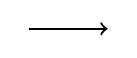
\begin{tikzpicture}
            \draw[->, thick] (0,0) -- (1,0);  % Draws an arrow
        \end{tikzpicture}
      \end{center}
    \end{column}
    \begin{column}{0.45\textwidth}
      \begin{center}
        Coloured graph:

        \includegraphics[height=30mm]{images/texpl_img/graph_coloured.png}
      \end{center}    
    \end{column}
  \end{columns}
\end{frame}

\begin{flashcardcpmpy}
\begin{frame}{Running Example -- CPMpy}
  \begin{example}[Graph Colouring]
    \footnotesize	
    Graph colouring is the problem of assigning colours to the nodes of a graph, such that no two \textbf{adjacent} nodes share the same colour. 

    \footnotesize\lstinputlisting[language=cpmpy,numbers=none,firstline=15,lastline=19]{models_cpmpy/t3_graph_colouring.py}    
  \end{example}

  \vspace{-0.4cm}
  \footnotesize	
  \begin{columns}
    \begin{column}{0.45\textwidth}
      \begin{center}
        Initial graph:

        \includegraphics[height=30mm]{images/texpl_img/graph_not_coloured.png}
      \end{center}
    \end{column}
    \begin{column}{0.1\textwidth}
      \begin{center}
        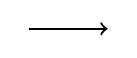
\begin{tikzpicture}
          \draw[->, thick] (0,0) -- (1,0);  % Draws an arrow
        \end{tikzpicture}
      \end{center}
    \end{column}
    \begin{column}{0.45\textwidth}
      \begin{center}
        Coloured graph:

        \includegraphics[height=30mm]{images/texpl_img/graph_coloured.png}
      \end{center}    
    \end{column}
  \end{columns}
\end{frame}
\end{flashcardcpmpy}


\subsection{General case: Explaining unsatisfiabilty}

\begin{frame}{Graph Colouring: Unsatisfiable}
    But what if our problem is not satisfiable?
    \begin{itemize}
        \item e.g. we have less colours available than needed!
    \end{itemize}
    \begin{example}
      \texttt{m, nodes = graph\_coloring(G, max\_colors=3)}
      
      \texttt{No solution found.}
    \end{example}
    \vfill

    Explanation techniques can help us understand:
    \begin{itemize}
      \item Why is it unsatisfiable? (Deductive explanation) 
      \item How to fix it? (Counterfactual explanation)
    \end{itemize}
\end{frame}


\subsubsection{Deductive Explanations}

\begin{frame}{Deductive  Explanations}
  \begin{columns}
    \begin{column}{0.5\textwidth}
      \begin{center}
        \includegraphics[height=60mm]{images/texpl_img/explain_unsat.png}
      \end{center}        
    \end{column}
    \begin{column}{0.5\textwidth}
      \begin{itemize}
        \item Find the cause!
        \item Why $X$? (e.g. why is it UNSAT?)
      \end{itemize}
    \end{column}
  \end{columns}    
\end{frame}

\begin{frame}{Deductive Explanations}
  \begin{center}
    Question: "Why is it unsatisfiable?"
  \end{center}
  \begin{columns}
    \begin{column}{0.5\textwidth}
      \begin{itemize}
        \item Answer: "The set of all constraints cannot be satisfied."
      \end{itemize}
      \begin{center}
        \includegraphics[height=30mm]{images/texpl_img/allcons.png}
      \end{center}

      Not very useful ...
      \vfill
    \end{column}    
    \begin{column}{0.5\textwidth}
      \begin{itemize}  
        \item Answer: "This (small) subset of constraints cannot be satisfied together!"
      \end{itemize}
      \begin{center}
        \includegraphics[height=30mm]{images/texpl_img/mus.png}
      \end{center}
      
      Pinpoint to a subset of constraints causing a conflict ... 
      \vfill
    \end{column}    
  \end{columns}
\end{frame}

\begin{frame}{Deductive Explanations: Graph colouring}
  \begin{center}
    Question: "Why is my graph colouring problem unsatisfiable?"
  \end{center}
  \begin{columns}
    \begin{column}{0.5\textwidth}
      \begin{itemize}
        \item Answer: "I cannot colour this graph with all these constraints."
      \end{itemize}
      \begin{center}
        \includegraphics[height=30mm]{images/texpl_img/graph_all_cons_red.png}
      \end{center}

      Not very useful ...
      \vfill
    \end{column}    
    \begin{column}{0.5\textwidth}
      \begin{itemize}  
        \item Answer: "These constraints prevent me from finding a solution!"
      \end{itemize}
      \begin{center}
        \includegraphics[height=30mm]{images/texpl_img/graph_mus_red.png}
      \end{center}

      Pinpoint to the subset of constraints causing a conflict ... 
    \end{column}    
  \end{columns}
\end{frame}

\begin{frame}{Deductive Explanations: Nurse Rostering}
  \begin{center}
    Question: "Why is my nurse rostering problem unsatisfiable?"
  \end{center}
  \begin{columns}
    \begin{column}{0.5\textwidth}
      \begin{itemize}
        \item Answer: "I cannot schedule satisfying all these constraints."
      \end{itemize}
      \begin{center}
        \includegraphics[height=30mm]{images/texpl_img/nr_all.png}
      \end{center}

      Not very useful ...
      \vfill
    \end{column}    
    \begin{column}{0.5\textwidth}
      \begin{itemize}  
        \item Answer: "These constraints prevent me from finding a solution!"
      \end{itemize}
      \begin{center}
        \includegraphics[height=30mm]{images/texpl_img/nr_mus.png}
      \end{center}

      Pinpoint to the subset of constraints causing a conflict ... 
      \vfill
    \end{column}    
  \end{columns}
\end{frame}

\begin{frame}{Minimal Unsatisfiable Subset (MUS)}
  The cause of UNSAT: A set of constraints that cannot be satisfied in conjunction! 

  \begin{center}
    \includegraphics[height=30mm]{images/texpl_img/mus.png}
  \end{center}

  \begin{definition}[Minimal Unsatisfiable subset (MUS)]
    A subset of constraints $C^{\prime} \subseteq C$ is called a MUS of $C$ if:
    \begin{itemize}
      \item $C^{\prime}$ is unsatisfiable, i.e., $solve(C^{\prime}) = UNSAT$.
      \item $C^{\prime}$ is minimal, i.e., $\forall c \in C^{\prime}$, $solve(C^{\prime} \setminus \{c\}) = SAT $ .
    \end{itemize}
  \end{definition}
\end{frame}

\begin{frame}{Minimal Unsatisfiable Subset (MUS)}
  The cause of UNSAT: A set of constraints that cannot be satisfied in conjunction! 

  \begin{center}
    \includegraphics[height=30mm]{images/texpl_img/mus.png}

    \begin{itemize}
      \item Explain the cause.
      \item Pinpoint to constraints causing a conflict.
      \item Trim model to a minimal set of constraints.
      \item Minimize cognitive burden for user.
    \end{itemize}      
  \end{center}
\end{frame}

\begin{frame}{Minimal Unsatisfiable Subset (MUS)}
  A cause of UNSAT: A set of constraints that cannot be satisfied in conjunction! 

  \begin{center}
    \includegraphics[height=30mm]{images/texpl_img/mus.png}

    \begin{itemize}
      \item Explain a cause. \alert{Important! Explain one of the (possibly many) causes}
      \item Pinpoint to constraints causing a conflict.
      \item Trim model to a minimal set of constraints.
      \item Minimize cognitive burden for user.
    \end{itemize}      
  \end{center}
\end{frame}

\begin{frame}{Computing MUSes}
  Multiple ways to compute MUSes. Deletion-based MUS algorithm:
  \vfill

  \begin{center}
    \includegraphics[height=35mm]{images/texpl_img/mus_naive_diagram.png}
  \end{center}
\end{frame}

\begin{flashcardcpmpy}
\begin{frame}{Computing MUSes -- CPMpy}
  Multiple ways to compute MUSes. Deletion-based MUS algorithm:

  \begin{example}[Deletion-based MUS algorithm]
    \footnotesize\lstinputlisting[language=cpmpy,firstline=4,lastline=16]{models_cpmpy/mus_naive.py}
  \end{example}
\end{frame}
\end{flashcardcpmpy}

\begin{frame}{Computing MUSes}
  Deletion-Based MUS - Example:

  \begin{center}
    \includegraphics[height=60mm]{images/texpl_img/del-based-mus.png}
  \end{center}
\end{frame}

\begin{frame}{Computing MUSes}
  \begin{itemize}
    \item Simple deletion-based approach is the baseline
          \vfill \vfill

    \item Use Assumption-based solving.
          \begin{itemize}
            \item Extract UNSAT core from solver ... and exploit incremental solving!
          \end{itemize}
          \vfill \vfill

    \item Divide-and-conquer approach $\xrightarrow{}$ QuickXplain.
          \begin{itemize}
            \item Binary search: remove half the constraints for each check
          \end{itemize}
          \vfill \vfill

  \end{itemize}
\end{frame}

\begin{flashcardcpmpy}
\begin{frame}{Computing MUSes -- CPMpy}
  \begin{itemize}
    \item Simple deletion-based approach is the baseline
          \begin{example}
            \cpminline{from cpmpy.tools.explain.mus import mus_naive}
          \end{example}   

    \item Use Assumption-based solving.
          \begin{itemize}
            \item Extract UNSAT core from solver ... and exploit incremental solving!
          \end{itemize}
          \begin{example}
            \cpminline{from cpmpy.tools.explain.mus import mus}
          \end{example}    
    \item Divide-and-conquer approach $\xrightarrow{}$ QuickXplain.
          \begin{itemize}
            \item Binary search: remove half the constraints for each check
          \end{itemize}
          \begin{example}
            \cpminline{from cpmpy.tools.explain.mus import quickxplain}
          \end{example}
  \end{itemize}
\end{frame}
\end{flashcardcpmpy}

\begin{frame}{Which MUS to return?}
  Multiple MUSes may exist! 

  The nurse rostering problem we saw has 100k+ MUSes!
  \begin{center}
    \includegraphics[height=60mm]{images/texpl_img/musses.png}
  \end{center}
\end{frame}

\begin{frame}{Which MUS to return?}
  Multiple MUSes may exist! 

  The nurse rostering problem we saw has 100k+ MUSes!
  \begin{itemize}
    \item Which one to show?
    \item Smaller MUSes may be more \textbf{understandable}.
    \item Some MUSes may involve more \textbf{understandable} constraints than others.
    \item Can we influence which MUS to find and show?
  \end{itemize}
\end{frame}

\begin{frame}{Which MUS to return?}
  \begin{definition}[Optimal Unsatisfiable Subset (OUS)]
    Given a set of constraints $C$, with each constraint associated with a weight, an OUS is a MUS $C^{\prime} \subseteq C$ that minimizes the sum of weights: \textit{min} $\sum_{c_i \in C^{\prime}} w_i \cdot c_i$.
  \end{definition}

  Based on the fact that some constraints may be \inference{easier to understand} than others!
  \vfill

  \begin{definition}[Smallest Unsatisfiable Subset (sMUS)]
    Given a set of constraints $C$, an sMUS is a Minimal Unsatisfiable Subset $C^{\prime} \subseteq C$ that minimizes the cardinality: \textit{minimize} $|C^{\prime}|$. An sMUS is an OUS in the case that all constraints have equal weights.
  \end{definition}

  Typically, in explanations also \blue{smaller is better}: Explaining with the fewest constraints is possibly good enough!
\end{frame}

\begin{frame}{Key concepts used for finding optimal MUSes}

  \begin{definition}[Maximal Satisfiable Subset (MSS)]
    Given a set of constraints $C$, an MSS is a subset $C^{\prime} \subseteq C$ that is satisfiable and maximal, meaning there is no constraint $c \in C \setminus C^{\prime}$ such that $C^{\prime} \cup \{c\}$ remains satisfiable.
  \end{definition}
  \vfill

  \begin{definition}[Minimal Correction Subset (MCS)]
    Given a set of constraints $C$, an MCS is a subset $C^{\prime} \subseteq C$ that is minimal such that $C \setminus C^{\prime}$ is satisfiable. In other words, an MCS is a smallest subset of constraints whose removal results in a Maximal Satisfiable Subset (MSS).
  \end{definition}
  \vfill

  \begin{center}
    \includegraphics[height=25mm]{images/texpl_img/mcs.png}
  \end{center}
\end{frame}

\begin{frame}{Key concepts used for finding optimal MUSes}

  \begin{definition}[Hitting Set]
    Given a collection of sets \( \mathcal{S} = \{S_1, S_2, \dots, S_n\} \), a hitting set is a subset \( H \subseteq \bigcup_{i=1}^n S_i \) such that \( H \cap S_i \neq \emptyset \) for every \( S_i \in \mathcal{S} \). In other words, a hitting set contains at least one element from each set in the collection.
  \end{definition}
  \vfill

  \begin{definition}[Hitting set duality]
    A MUS is a hitting set of all MCSes, and an MCS is a hitting set of all MUSes. 

    Let $M$ be the collection of all MUSes, and $S$ be the collection of all MCSes.

    \begin{itemize}
      \item Every MUS $M_i \in M$ is a hitting set of all MCSes $S$: $\forall S_j \in S$, $M_i \cap S_j \neq \emptyset$.
      \item Every MCS $S_j \in S$ is a hitting set of all MUSes $M$: $\forall M_i \in M$, $S_j \cap M_i \neq \emptyset$.
    \end{itemize}
  \end{definition}
\end{frame}

\begin{frame}{Key concepts used for finding optimal MUSes}

  \begin{definition}[Hitting set duality]
    A MUS is a hitting set of all MCSes, and an MCS is a hitting set of all MUSes. 

    Let $M$ be the collection of all MUSes, and $S$ be the collection of all MCSes.
    \begin{itemize}
      \item Every MUS $M_i \in M$ is a hitting set of all MCSes $S$: $\forall S_j \in S$, $M_i \cap S_j \neq \emptyset$.
      \item Every MCS $S_j \in S$ is a hitting set of all MUSes $M$: $\forall M_i \in M$, $S_j \cap M_i \neq \emptyset$.
    \end{itemize}
  \end{definition}

  \vfill
  \begin{columns}

    \begin{column}{0.5\textwidth}        
      \begin{center}
        \includegraphics[height=30mm]{images/texpl_img/mus.png}
      \end{center}
    \end{column}

    \begin{column}{0.5\textwidth}        
      \begin{center}
        \includegraphics[height=30mm]{images/texpl_img/hittingset.png}
      \end{center}
    \end{column}
  \end{columns}
\end{frame}

\begin{frame}{Optimizing which MUS is found}
  Find all MUSes, and pick the best? 
  \red{NO!} Potentially exponential number of MUSes
  \vfill

  \begin{center}
    \includegraphics[height=62mm]{images/texpl_img/ocus.png}
  \end{center}
\end{frame}

\begin{frame}{Optimizing which MUS is found}
  Find all MUSes, and pick the best? 
  \red{NO!} Potentially exponential number of MUSes
  \vfill

  \begin{center}
    \includegraphics[height=52mm]{images/texpl_img/ocus_algo.png}
  \end{center}
\end{frame}

\begin{flashcardcpmpy}
\begin{frame}{Finding optimal MUSes -- CPMpy}

  OCUS algorithm for finding the optimal MUS:
  \begin{example}
    \cpminline{from cpmpy.tools.explain.mus import optimal_mus}\\
    \cpminline{optimal_mus(constraints, weights=...)}
  \end{example}
  \vfill

  OCUS algorithm for finding the smallest MUS (default weights are equal):
  \begin{example}
    \cpminline{from cpmpy.tools.explain.mus import optimal_mus}\\
    \cpminline{optimal_mus(constraints)}\\
  \end{example}    
  \vfill

  Can directly use \cpminline{smus}, which uses \cpminline{optimal_mus} as above: 
  \begin{example}        
    \cpminline{from cpmpy.tools.explain.mus import smus}\\
    \cpminline{smus(constraints)}\\
  \end{example}    
\end{frame}
\end{flashcardcpmpy}


\subsubsection{Counterfactual Explanations}

\begin{frame}{Counterfactual explanations}

  Not always enough to explain the cause!
  \vspace{-0.5cm}
  \begin{columns}
    \begin{column}{0.75\textwidth}
      How to \textbf{change the model}, in order to find a solution?
      \vfill

      \begin{itemize}
        \item Find constraints that, if \textit{removed}, a solution can be found!
        \item Find a correction subset \dots
      \end{itemize}
    \end{column}
    \begin{column}{0.3\textwidth}
      \begin{center}
        "Removing this constraint will make our problem satisfiable"
        \includegraphics[height=25mm]{images/texpl_img/graph_mcs_red.png}
      \end{center}
    \end{column}
  \end{columns}


  Reminder: 
  \begin{definition}[Minimal Correction Subset (MCS)]
    Given a set of constraints $C$, an MCS is a subset $C^{\prime} \subseteq C$ that is minimal such that $C \setminus C^{\prime}$ is satisfiable. In other words, an MCS is a smallest subset of constraints whose removal results in a Maximal Satisfiable Subset (MSS).
  \end{definition}
\end{frame}

\begin{frame}{Computing MCSes}

  MCSes can be used to provide counterfactual explanations \dots How to compute them?
  \vfill

  \begin{columns}
    \begin{column}{0.5\textwidth}
      \textbf{Key property}: \\MCSes are the complement of MSSes!!
      \begin{center}
        \includegraphics[height=25mm]{images/texpl_img/mcs.png}
      \end{center}
    \end{column}

    \begin{column}{0.5\textwidth}
      Grow a set of constraints $C^{\prime} \subseteq C$ until UNSAT! \textbf{Take the complement}.
      \begin{center}
        \includegraphics[height=25mm]{images/texpl_img/mcs_grow.png}
      \end{center}
    \end{column}
  \end{columns}
\end{frame}

\begin{flashcardcpmpy}
\begin{frame}{Computing MCSes -- CPMpy}
  Simple growing-based approach (similar to deletion-based MUS):

  \begin{example}[Grow-based MCS/MSS]
    \footnotesize\lstinputlisting[language=cpmpy,numbers=none,firstline=3, lastline=13]{models_cpmpy/mcs_naive.py}   
  \end{example}

  $\xrightarrow{}$ Finds any MSS/any MCS!\\
  $\xrightarrow{}$ Many may exist!
\end{frame}
\end{flashcardcpmpy}

\begin{frame}{Computing optimal MCSes}
    
  Maximize the number of satisfied constraints \dots treat it as (weighted) MAX-CSP!

  $\xrightarrow{}$ One \textit{optimization} problem, instead of multiple \textit{satisfaction} ones \dots

  $\xrightarrow{}$ MAX-CSP: Find a solution that satisfies a maximum number of constraints.

  $\xrightarrow{}$ Finds largest MSS = complement of smallest MCS!
  \vspace{0.3cm}
  \vfill

  \begin{itemize}
    \item (Half-)Reify all constraints in $C$, creating boolean indicator variables for each: 
          $$b_i \xrightarrow{} c_i, \forall c_i \in C$$
          \vspace{-0.3cm}
    
    \item and maximize the sum of the values of reification variables:
          $$\text{maximize } \sum_{i=1}^{|C|} b_i$$
          \vspace{-0.3cm}

    \item Simply take the constraints not satisfied:
          $$MCS = \{ c_i \in C \mid \neg b_i \}$$
  \end{itemize}
\end{frame}

\begin{flashcardcpmpy}
\begin{frame}{Computing optimal MCSes -- CPMpy}
    
  Maximize the number of satisfied constraints \dots treat it as (weighted) MAX-CSP!

  $\xrightarrow{}$ One \textit{optimization} problem, instead of multiple \textit{satisfaction} ones \dots

  $\xrightarrow{}$ MAX-CSP: Find a solution that satisfies a maximum number of constraints.

  $\xrightarrow{}$ Finds largest MSS = complement of smallest MCS!
  \vspace{0.3cm}
  \vfill

  \begin{itemize}
    \item (Half-)Reify all constraints in $C$, creating boolean indicator variables for each: 
          \lstinputlisting[language=cpmpy,numbers=none,firstline=5, lastline=7]{models_cpmpy/mcs_opt.py}

    \item and maximize the sum of the values of reification variables:
          \lstinputlisting[language=cpmpy,numbers=none,firstline=9, lastline=10]{models_cpmpy/mcs_opt.py}

    \item Simply take the constraints not satisfied:
          \lstinputlisting[language=cpmpy,numbers=none,firstline=12, lastline=12]{models_cpmpy/mcs_opt.py}
  \end{itemize}
\end{frame}
\end{flashcardcpmpy}

\begin{frame}{Computing optimal MCSes}
    
  Maximize the number of satisfied constraints \dots treat it as (weighted) MAX-CSP!

  $\xrightarrow{}$ One \textit{optimization} problem, instead of multiple \textit{satisfaction} ones \dots

  $\xrightarrow{}$ MAX-CSP: Find a solution that satisfies a maximum number of constraints.

  $\xrightarrow{}$ Finds largest MSS = complement of smallest MCS!
  \vfill

  \textbf{Alternative}: 
  \begin{itemize}
    \item Let CPMpy handle the reification
    \item Use directly the (soft) constraints
  \end{itemize}

  \footnotesize\lstinputlisting[language=cpmpy,numbers=none,firstline=6, lastline=8]{models_cpmpy/mcs_opt2.py}
\end{frame}


\subsection{Explaining solutions and optimality}

\begin{frame}{Explaining solutions}
      
  "Why $X$?": Why is $X$ part of the solution?
  \vfill

  Explaining logical consequences:
  \begin{definition}[Logical consequence]
    Logical consequence: a variable assignment entailed by the constraints (and possible an initial partial assignment)
  \end{definition}
  \vfill

  Is $X$ a logical consequence? Try to solve the problem, enforcing $\neg X$:
  \begin{itemize}
    \item If \inference{SAT}: no explanation, return new solution.
    \item If \red{UNSAT}: use any technique for explaining this UNSAT problem (MUS, MCS, \dots).
  \end{itemize}
\end{frame}

\begin{frame}{Explaining optimality}
  "Why $X$?": Why this solution is optimal w.r.t. the objective function $f(x)$?
  \vfill

  Explaining logical consequences!
  \begin{itemize}
    \item Taking into account also the objective value found!
  \end{itemize}
  \vfill

  Try to solve the problem, enforcing $f(x) < o$ (assume minimization problem),\\ with $o$ being the objective value of the optimal solution:
  \begin{itemize}
    \item Will be \red{UNSAT}, as we know $o$ is optimal!
    \item Use any technique for explaining this UNSAT problem(MUS, MCS, \dots).
  \end{itemize}
\end{frame}

\begin{frame}{Explaining optimality}
    
  "Why $X$?": Why is this solution optimal w.r.t. the objective function $f(x)$?
  \vfill

  Graph colouring is actually an optimization problem!

  \begin{example}
    \footnotesize\lstinputlisting[language=cpmpy,numbers=none,firstline=16,lastline=20]{models_cpmpy/t3_graph_colouring.py}   
  \end{example}

  \begin{columns}
    \begin{column}{0.6\textwidth}
      \vspace{-0.5cm}
      \begin{center}
        Why does the best solution need 4 colours?
        \includegraphics[height=30mm]{images/texpl_img/graph_coloured.png}
      \end{center}
    \end{column}

    \begin{column}{0.5\textwidth}
      Because of these constraints!
      \vspace{-0.3cm}
      \begin{center}
        \includegraphics[height=30mm]{images/texpl_img/graph_mus_red.png}
      \end{center}
    \end{column}
  \end{columns}
\end{frame}


\section{Summary}

\begin{frame}{Summary}
  \begin{itemize}
    \item Model + \textbf{Solve}
          \begin{center}
            \includegraphics[height=40mm]{images/prob2sol.png}
          \end{center}

    \item Debugging a model
          \vfill

    \item Explainable Constraint Solving
  \end{itemize}
\end{frame}

\begin{frame}{Summary}
  \begin{itemize}
    \item Model + \textbf{Solve}
          \vfill

    \item Debugging a model
          \begin{center}
            \includegraphics[height=20mm]{images/texpl_img/debug.jpg}
          \end{center}
          \url{https://cpmpy.readthedocs.io/en/latest/how_to_debug.html}
          \vfill

    \item Explainable Constraint Solving
  \end{itemize}
\end{frame}


\begin{frame}{Summary}
  \begin{columns}
    \begin{column}{0.7\textwidth}
      \begin{itemize}
        \item Model + \textbf{Solve}
              \vspace{0.5cm}

        \item Debugging a model
              \vspace{0.5cm}

        \item Explainable Constraint Solving \vfill
        
              \includegraphics[height=20mm]{images/texpl_img/mus.png}
              $ $
              \includegraphics[height=20mm]{images/texpl_img/mcs_grow.png}
      \end{itemize} \vfill
      
      Advanced tutorial: \url{https://github.com/CPMpy/XCP-explain}
    \end{column}

    \begin{column}{0.3\textwidth}
      \begin{center}
        \includegraphics[height=50mm]{images/texpl_img/interaction_figure4.png}
      \end{center}
    \end{column}
  \end{columns}
\end{frame}

\end{document}
